\documentclass[a4paper, 11pt]{article}
\usepackage[ngerman]{babel}
%ä und so
\usepackage[utf8]{inputenc}
\usepackage[T1]{fontenc}
\usepackage{amsmath}
\usepackage{amsthm}
\usepackage{amsbsy}

\usepackage{mathrsfs}
\usepackage{amssymb}
\usepackage{amstext}
\usepackage{amsfonts}
\usepackage{float}
\usepackage{graphicx}
\usepackage{esdiff}
\usepackage{hyperref}
\usepackage{geometry}
\geometry{top = 20mm, bottom = 20 mm, left = 25mm, right = 25mm}


\usepackage{setspace}
\onehalfspacing

\usepackage{fancyhdr}
\usepackage{wrapfig}
%\usepackage[hyphens]{url}
%\urlstyle{sf}
%\usepackage[hidelinks]{hyperref}
%\usepackage{breakurl}
%\hypersetup{colorlinks=false}
\usepackage{multirow}

%\usepackage{svg}

\title{Optik I $\looparrowright\rightsquigarrow\multimap$ Prismen- und Gitterspektroskopie}
\author{Gruppe B14 \\ \\ Daniel Wendland \\ Philipp Bremer \\ Olexiy Fedorets \\ Jonathan Hermann}
\date{\today}

% !TeX spellcheck = de_DE
\begin{document}


\begin{titlepage}
\vspace*{\fill}
\begin{center}
	\vfill
	\newcommand{\Line}{\rule{\linewidth}{0.6mm}}
	\Line 
	{\let\newpage\relax\maketitle}
	\Line 
	\vfill
\end{center}
\vspace*{\fill}
\thispagestyle{empty}
\end{titlepage}





\newpage
\thispagestyle{empty}
\tableofcontents
\newpage

%Kopf- und Fußzeile
\pagestyle{fancy}
\fancyhf{}
%Kopfzeile links bzw. innen
\fancyhead[L]{\nouppercase{\leftmark}}
%Kopfzeile rechts bzw. außen
\fancyhead[R]{\thepage}
%Linie oben
\renewcommand{\headrulewidth}{0.5pt}
\fancyfoot[C]{\thepage}


\setcounter{page}{1}

\section{Gitterspektrometer}

\subsection{Theoretische Grundlagen der Gitterspektroskopie}

\begin{figure}[H]
	\centering
	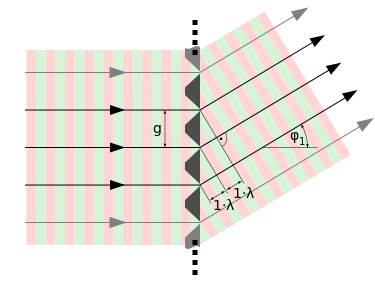
\includegraphics[scale=0.8]{./Bilder/Beugungsgitter-erstes-Maximum.png}
	\caption{Interferenz von ebenen Wellen am Gitter, mit Gangunterschied $\Delta=\lambda$ für das Maximum erster Ordnung \protect \footnotemark}
	\label{pic:Gitter}	
\end{figure}
\footnotetext{Quelle:Wikipedia - \url{https://commons.wikimedia.org/wiki/File:Beugungsgitter-erstes-Maximum.svg}}

Ein Gitter wird charakterisiert durch die Spaltbreite $b$, Gitterkonstante $d$ und die Anzahl der \textbf{ausgeleuchteten} Spalte $N$. Auf das Gitter treffen parallele, ebene Wellenfronten (\textit{Fraunhofer-Beugung}) und werden an den Spalten gebeugt, wobei jeder Punkt der Spaltöffnungen Ausgangspunkt einer gleichphasigen Kugelwelle ist (\textit{Huygenssches Prinzip}).

Für den Gangunterschied  der Teilwellen, die konstruktiv miteinander interferieren, lässt sich folgender Zusammenhang aufstellen:
\begin{equation}
	\Delta = g \cdot \sin(\varphi_n) = n \cdot \lambda
\end{equation}
In Abbildung \ref{pic:Gitter} ist dies für das Maximum erster Ordnung gezeigt.

Falls das Gitter jedoch nicht senkrecht zum Strahlengang ausgerichtet ist, muss zusätzlich der Gangunterschied \textbf{vor} dem Gitter berücksichtigt werden:
\begin{equation}
	n \cdot \lambda = g \cdot (\sin(\vartheta)+\sin(\phi_n-\vartheta))
\end{equation}
Hier ist jetzt $\phi_n$ der Winkel zwischen Einfallsstrahl und Beobachtungsrichtung und $\vartheta$ der Drehwinkel des Gitters zum Lot hin.

Es ergibt sich, dass die Lage der Intensitätsmaxima antiproportional zu Wellenlänge des Lichts ist. Der Beugungswinkel (also Linienabstand) ist antiproportional zum Spaltabstand.
Die Hauptmaxima des Gitters werden mit wachsender Spaltanzahl schmaler und steiler. Außerdem befinden sich zwischen diesen noch $N-2$ Nebenmaxima, deren Intensität jedoch mit $N^2$ abnimmt, wodurch diese im Versuch garnicht sichtbar sind.


\clearpage
\paragraph{Auflösungsvermögen}
Das spektrale Auflösungsvermögen des Gitters lässt sich mit Hilfe des \textit{Rayleigh-Kriteriums} herleiten und beträgt
\begin{equation}\label{eq:AGitter}
	A = \frac{\lambda}{\Delta\lambda} = n \cdot N
\end{equation}
Dabei nimmt man an, dass wir Spektrallinien genau dann noch trennen können, wenn das Maximum der ersten Linie im Minimum der zweiten liegt.




\subsection{Aufbau}
Der Aufbau des Gitterspektrometers ist analog zu dem vom Prismenspektrometer (ref), nur das jetzt ein Gitter in den Strahlengang gestellt wird. Dabei muss darauf geachtet werden, dass dieses senkrecht zum einfallenden Strahl steht, da sonst bereits vor dem Gitter ein Gangunterschied der Strahlen vorliegt und die Lage der Maxima sich dadurch verschiebt. Da dies mit den zur Verfügung stehenden Mitteln aber nicht sichergestellt werden kann, muss später bei der Auswertung untersucht werden, ob das Gitter schräg stand.

Außerdem wird bei diesem Versuch zusätzlich zur \texttt{HgCd}-Lampe eine \texttt{Na}-Lampe verwenden, um die Wellenlänge der Natrium-Doppellinie und Anhand dieser das Auflösungsvermögen des Gitters zu bestimmen.

Der gesamte Versuch wurde mit einem Gitter mit 600 Strichen$/mm$ durchgeführt.


\subsection{Durchführung}
Das grundlegende Vorgehen ist ähnlich zu dem beim Prismenspektrometer: durch Ausrichtung des Fernrohrs auf die einzelnen Spektrallinien und Ablesen des Nonius werden die Beugungswinkel vermessen.

Zu Beginn wird die Nulllinie (Maximum 0.-Ordnung) der \texttt{HgCd}-Lampe durch 10-fache Messung bestimmt. Es wird angenommen, dass der statistische Fehler auf die folgenden Messungen gleich bleibt, daher werden die Linien im folgenden nurnoch 3 Mal ausgemessen.

\begin{equation}
*Nulllinie*	
\end{equation}

\subsubsection{Bestimmung der Gitterkonstante}
Zunächst werden die Wellenlängen der Spektrallinien der \texttt{HgCd}-Lampe als bekannt angenommen (diese stammen aus der \texttt{NIST}-Datenbank und haben nur sehr geringe Unsicherheiten, und werden daher als nicht fehlerbehaftet angenommen) und die Beugungswinkel $\phi_n$ werden gemessen. Dabei konnte nur bis zur zweiten Ordnung beobachtet werden. Leider konnten aus Zeitgründen nur 4 Spektrallinien (die am besten sichtbarsten) vermessen, die in Tabelle \ref{table:SpektrumHgCd} dargestellt sind. Die Winkel wurden immer 3 Mal gemessen und gemittelt, jeweils bis zur zweiten Ordnung auf beiden Seiten.

\begin{table}[H]
\large
\centering
	\begin{tabular}{|c|c|c|}
	\hline
	Element & Wellenlänge $[nm]$ & Farbe \\
	\hline
	Cd & 467,81 & blau \\
	\hline
	Cd & 508,58 & grün \\
	\hline
	Hg & 576,96 & gelb \\
	\hline
	Cd & 643,85 & rot \\
	\hline
	\end{tabular}
\caption{Zur Vermessung ausgewählte Spektrallinien der \texttt{HgCd}-Lampe (Werte stammen aus der \texttt{NIST}-Datenbank)}
\label{table:SpektrumHgCd}
\end{table}

Der Beugungswinkel ist dabei immer die Differenz des gemessenen Winkels und der Nulllinie. Aus den Winkel kann dann durch eine lineare Regression die Gitterkonstante bestimmt werden.

\subsubsection{Bestimmung der Wellenlängen der \texttt{Na}-Doppellinie}
Mit Hilfe der Zuvor bestimmten Gitterkonstante wird nun die Natrium-Doppellinie ausgemessen. Auch hier wurde bis zur zweiten Ordnung auf beiden Seiten 3 Mal gemessen und gemittelt.


Die ermittelten Werte werden mit den realen Werte in Tabelle \ref{table:SpektrumNa} verglichen.

\begin{table}[H]
	\large
	\centering
	\begin{tabular}{|c|c|}
		\hline
		Wellenlänge $[nm]$ & Farbe \\
		\hline
		589,59 & gelb \\
		\hline
		589,00 & gelb \\
		\hline
	\end{tabular}
	\caption{\texttt{Na}-Doppellinie (Werte stammen aus der \texttt{NIST}-Datenbank)}
	\label{table:SpektrumNa}
\end{table}

\subsubsection{Bestimmung des Auflösungsvermögens}
Das Auflösungsvermögen des Gitters wird auch anhand der \texttt{Na}-Doppellinie bestimmt (dieses ist unabhängig von Wellenlänge oder Gitterkonstante! \ref{eq:AGitter}).
Um die Abhängigkeit von der Anzahl $N$ der ausgeleuchteten Spalte zu realisieren, wird eine Schlitzblende verwendet, die feste Schlitzbreiten von $0,5mm$ bis $6mm$ in $0,5mm$-Schritten bietet. Es wird beobachtet, bei welcher Schlitzbreite die Doppellinie nicht mehr unterscheidbar wird. Dieses Ergebnis wird dann mit dem nach der Formel erwarteten Auflösungsvermögen ($A=589nm/0,59nm\approx998.3$) verglichen.



\clearpage
\subsection{Auswertung}
\paragraph{Bestimmung der Beugungswinkel}
\begin{equation}
	\varphi_n = \alpha - \varphi_0
\end{equation}
\subsubsection{Bestimmung der Gitterkonstante}


\subsubsection{Bestimmung der Wellenlängen der \texttt{Na}-Doppellinie}


\subsubsection{Bestimmung des Auflösungsvermögens}






\newpage
\listoffigures
\listoftables

\end{document}